\documentclass[border=4pt]{standalone}
% Shared style for FORGE paper figures (standalone, vector PDF)
\usepackage[T1]{fontenc}
\usepackage{lmodern}      % Latin Modern sans serif for diagrams
\renewcommand{\familydefault}{\sfdefault}
\usepackage{microtype}
\DisableLigatures[-]{encoding=T1,family=tt*}  % keep -- as two hyphens in CLI flags
\usepackage{textcomp}
\usepackage{amsmath}
\usepackage{tikz}
\usetikzlibrary{arrows.meta,positioning,calc,fit,backgrounds,shapes.geometric,shapes.misc,decorations.pathreplacing}

% ---- Moderate accent palette -------------------------------------------------
\definecolor{ink}{HTML}{222831}        % near-black text/borders
\definecolor{subink}{HTML}{5B6470}     % secondary text
\definecolor{accInput}{HTML}{2F5C9E}   % blue  -> plugin inputs
\definecolor{accModel}{HTML}{2A9D8F}   % teal  -> validated model / core
\definecolor{accGen}{HTML}{D7892B}     % amber -> generators / outputs
\definecolor{accVerif}{HTML}{6A4C93}   % purple-> verification
\definecolor{accMuted}{HTML}{8A94A3}   % grey  -> not-exercised / external

\colorlet{fillInput}{accInput!10}
\colorlet{fillModel}{accModel!14}
\colorlet{fillGen}{accGen!14}
\colorlet{fillVerif}{accVerif!12}
\colorlet{fillMuted}{accMuted!14}
\colorlet{fillPlain}{black!4}

% ---- Node styles -------------------------------------------------------------
\tikzset{
  font=\sffamily,
  >={Stealth[length=2.6mm,width=2.0mm]},
  base/.style={
    rounded corners=2pt, draw, line width=0.7pt,
    align=center, inner sep=5pt, text=ink,
    minimum height=10mm, font=\small},
  inbox/.style   ={base, draw=accInput, fill=fillInput},
  modelbox/.style={base, draw=accModel, fill=fillModel, line width=1.0pt},
  genbox/.style  ={base, draw=accGen,   fill=fillGen},
  verbox/.style  ={base, draw=accVerif, fill=fillVerif},
  mutedbox/.style={base, draw=accMuted, fill=fillMuted, text=subink},
  outbox/.style  ={base, draw=ink!55,   fill=fillPlain},
  title/.style   ={font=\bfseries\small, text=ink},
  grouptitle/.style={font=\bfseries\footnotesize, text=#1},
  lbl/.style     ={font=\scriptsize, text=subink, inner sep=2pt},
  flow/.style    ={draw=ink!70, line width=0.9pt, ->},
  flowmuted/.style={draw=accMuted, line width=0.8pt, ->, densely dashed},
  flowmodel/.style={draw=accModel, line width=1.1pt, ->},
  groupbg/.style ={rounded corners=4pt, draw=#1!55, line width=0.7pt,
                   fill=#1!5, dash pattern=on 3pt off 2pt},
}

\begin{document}
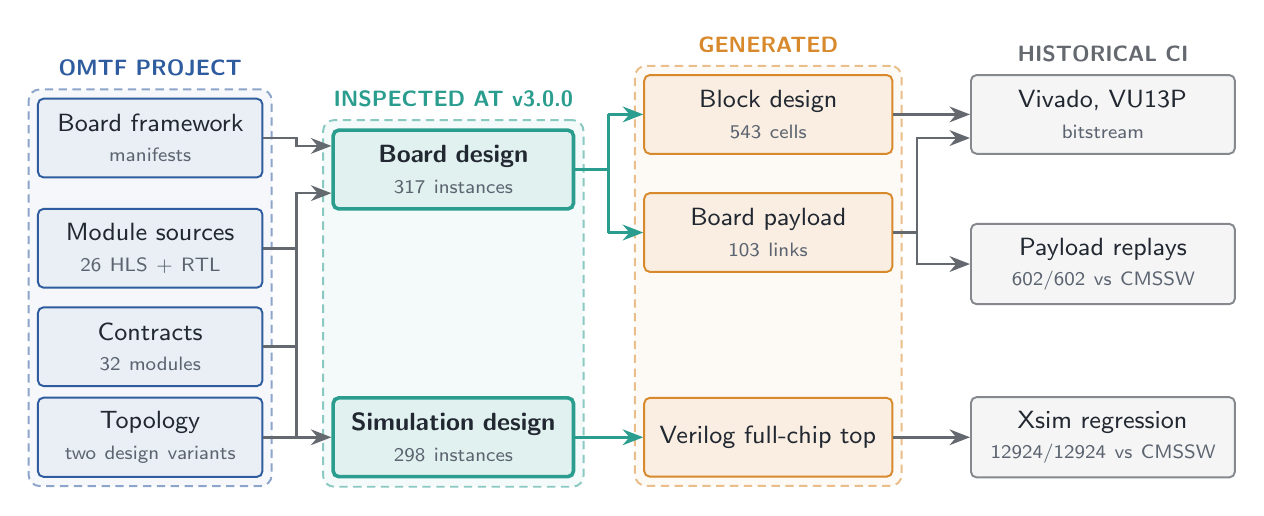
\begin{tikzpicture}
\def\colA{25mm}\def\colB{27mm}\def\colC{28mm}\def\colD{30mm}
\def\xB{38.5mm}\def\xC{78.5mm}\def\xD{121mm}

% ---- OMTF project inputs ----------------------------------------------------------
\node[inbox, text width=\colA] (f) at (0,0)
  {Board framework\\{\scriptsize\color{subink}manifests}};
\node[inbox, text width=\colA] (m) at (0,-14mm)
  {Module sources\\{\scriptsize\color{subink}26 HLS + RTL}};
\node[inbox, text width=\colA] (k) at (0,-26.5mm)
  {Contracts\\{\scriptsize\color{subink}32 modules}};
\node[inbox, text width=\colA] (t) at (0,-38mm)
  {Topology\\{\scriptsize\color{subink}two design variants}};

% ---- FORGE v3.0.0: two resolved designs ---------------------------------------------
\node[modelbox, text width=\colB, line width=1.3pt] (ir1) at (\xB,-4mm)
  {\textbf{Board design}\\{\scriptsize\color{subink}317 instances}};
\node[modelbox, text width=\colB, line width=1.3pt] (ir2) at (\xB,-38mm)
  {\textbf{Simulation design}\\{\scriptsize\color{subink}298 instances}};

% ---- Generated ----------------------------------------------------------------------
\node[genbox, text width=\colC] (bd) at (\xC,3mm)
  {Block design\\{\scriptsize\color{subink}543 cells}};
\node[genbox, text width=\colC] (p) at (\xC,-12mm)
  {Board payload\\{\scriptsize\color{subink}103 links}};
\node[genbox, text width=\colC] (v) at (\xC,-38mm)
  {Verilog full-chip top};

% ---- Checked by the project's continuous integration ---------------------------------
\node[outbox, text width=\colD] (rv) at (\xD,3mm)
  {Vivado, VU13P\\{\scriptsize\color{subink}bitstream}};
\node[outbox, text width=\colD] (rp) at (\xD,-16mm)
  {Payload replays\\{\scriptsize\color{subink}602/602 vs CMSSW}};
\node[outbox, text width=\colD] (rx) at (\xD,-38mm)
  {Xsim regression\\{\scriptsize\color{subink}12924/12924 vs CMSSW}};

% ---- Groups -------------------------------------------------------------------------
\begin{scope}[on background layer]
  \node[groupbg=accInput, fit=(f)(t), inner sep=3pt] (g1) {};
  \node[groupbg=accModel, fit=(ir1)(ir2), inner sep=3pt] (g2) {};
  \node[groupbg=accGen, fit=(bd)(v), inner sep=3pt] (g3) {};
\end{scope}
\node[grouptitle=accInput, above=1pt of g1.north] {OMTF PROJECT};
\node[grouptitle=accModel, above=1pt of g2.north] {INSPECTED AT v3.0.0};
\node[grouptitle=accGen, above=1pt of g3.north] {GENERATED};
\node[grouptitle=ink!70, above=1pt of rv.north] {HISTORICAL CI};

% ---- Flows --------------------------------------------------------------------------
\draw[flow] (f.east) -- (f.east -| g1.east) -- ++(3mm,0) |- ($(ir1.west)+(0,3mm)$);
\coordinate (j1) at ($(g1.east)+(3mm,0)$);
\foreach \n in {m,k,t} { \draw[draw=ink!70, line width=0.9pt] (\n.east) -- (j1 |- \n); }
\draw[draw=ink!70, line width=0.9pt] (j1 |- m) -- (j1 |- t);
\draw[flow] (j1 |- m) |- ($(ir1.west)+(0,-3mm)$);
\draw[flow] (j1 |- t) -- (ir2.west);

\coordinate (j2) at ($(g2.east)+(3mm,0)$);
\draw[accModel, line width=1.1pt] (ir1.east) -- (j2 |- ir1);
\draw[accModel, line width=1.1pt] (j2 |- bd) -- (j2 |- p);
\foreach \n in {bd,p} { \draw[flowmodel] (j2 |- \n) -- (\n.west); }
\draw[flowmodel] (ir2.east) -- (v.west);

\draw[flow] (bd.east) -- (rv.west);
\draw[flow] (p.east) -- ++(3mm,0) |- ($(rv.west)+(0,-3mm)$);
\draw[flow] (p.east) -- ++(3mm,0) |- (rp.west);
\draw[flow] (v.east) -- (rx.west);

\end{tikzpicture}
\end{document}
